\begin{sectionblock}{DoenetML}

  \begin{wrapfigure}{L}{0.4\textwidth}
    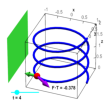
\includegraphics[width=0.38\textwidth]{vector-field.pdf}
  \end{wrapfigure}
  Interactives can be built via DoenetML, an opinionated markup
  language built to encode learner interactions with mathematical
  content.  Starting with primitives like \texttt{<point>}, complex
  interactives can be described and then shared with learners.

\end{sectionblock}

\vspace{1ex}

\begin{sectionblock}{Doenet API}
  Webpages, whether or not they are written using DoenetML, can use
  the Doenet API to record events.  These events can be analyzed to
  understand how engagement with the webpage affects learning.
  
\end{sectionblock}

\vspace{1ex}

\begin{sectionblock}{Join the Ongoing Work}
  Instructors, curriculum designers, technologists, and educational
  researchers will be brought together at Doenet workshops to
  collaborate.

  \vspace{1ex}Contact us at \texttt{info@doenet.org} to join the
  ongoing effort.
\end{sectionblock}


